\documentclass[10pt,xcolor={usenames,dvipsnames}]{beamer}
\graphicspath{{pics/}}
\fontfamily{pnc}
\usepackage{verbatim}
\usepackage{listings}

\title{Final Presentation}
\subtitle{MyTaxiService}
\author{Roberto Clapis, Erica Stella}
\institute{Politecnico di Milano}
\date{12/02/2016}
\subject{Software Engineering 2}

\usepackage{graphicx}
\usebackgroundtemplate{
\includegraphics[width=\paperwidth,height=\paperheight]{background2.jpg}}

\setbeamertemplate{navigation symbols}{}
\setbeamercolor{frametitle}{fg=CornflowerBlue}
\setbeamercolor{title}{fg=CornflowerBlue}
\setbeamercolor{framesubtitle}{fg=RoyalBlue}

\addtobeamertemplate{frametitle}{\vskip+3ex}{} 

\begin{document}
\frame{\titlepage}
\begin{frame}
	\frametitle{Table of Contents}
	\tableofcontents[currentsection]
\end{frame}


\section[Section]{RASD}

\begin{frame}
	\begin{center}
		RASD	
	\end{center}
\end{frame}
\begin{frame}
	\frametitle{The RASD Document}
	\framesubtitle{The approach}
	We tried to solve all the easy problems with a KISS approach, in order to focus on the actual difficulties. \\
	\begin{itemize}
		\item Login, logout, registration were kept as standard as possible
		\item Usability was kept in mind, customizability was not considered as a feature
		\item We tried to keep as little as possible the user inputs and let the application do the work
	\end{itemize}
\end{frame}
%TODO questi sono davvero troppi, non ha senso è un muro di testo
%\begin{frame}
%	\frametitle{Requirements}
%	\framesubtitle{Non functional requirements}
%	%TODO
%\end{frame}
%\begin{frame}
%	\frametitle{Requirements}
%	\framesubtitle{Functional requirements}
%	%TODO
%\end{frame}
%\begin{frame}
%	\frametitle{Domain Assumptions}
%	%TODO 
%\end{frame}
\begin{frame}
	\frametitle{Two simple interfaces}
	\framesubtitle{Adaptive web-based UI to ensure maintainability for both the web UI and mobile UI}
	\begin{center}
		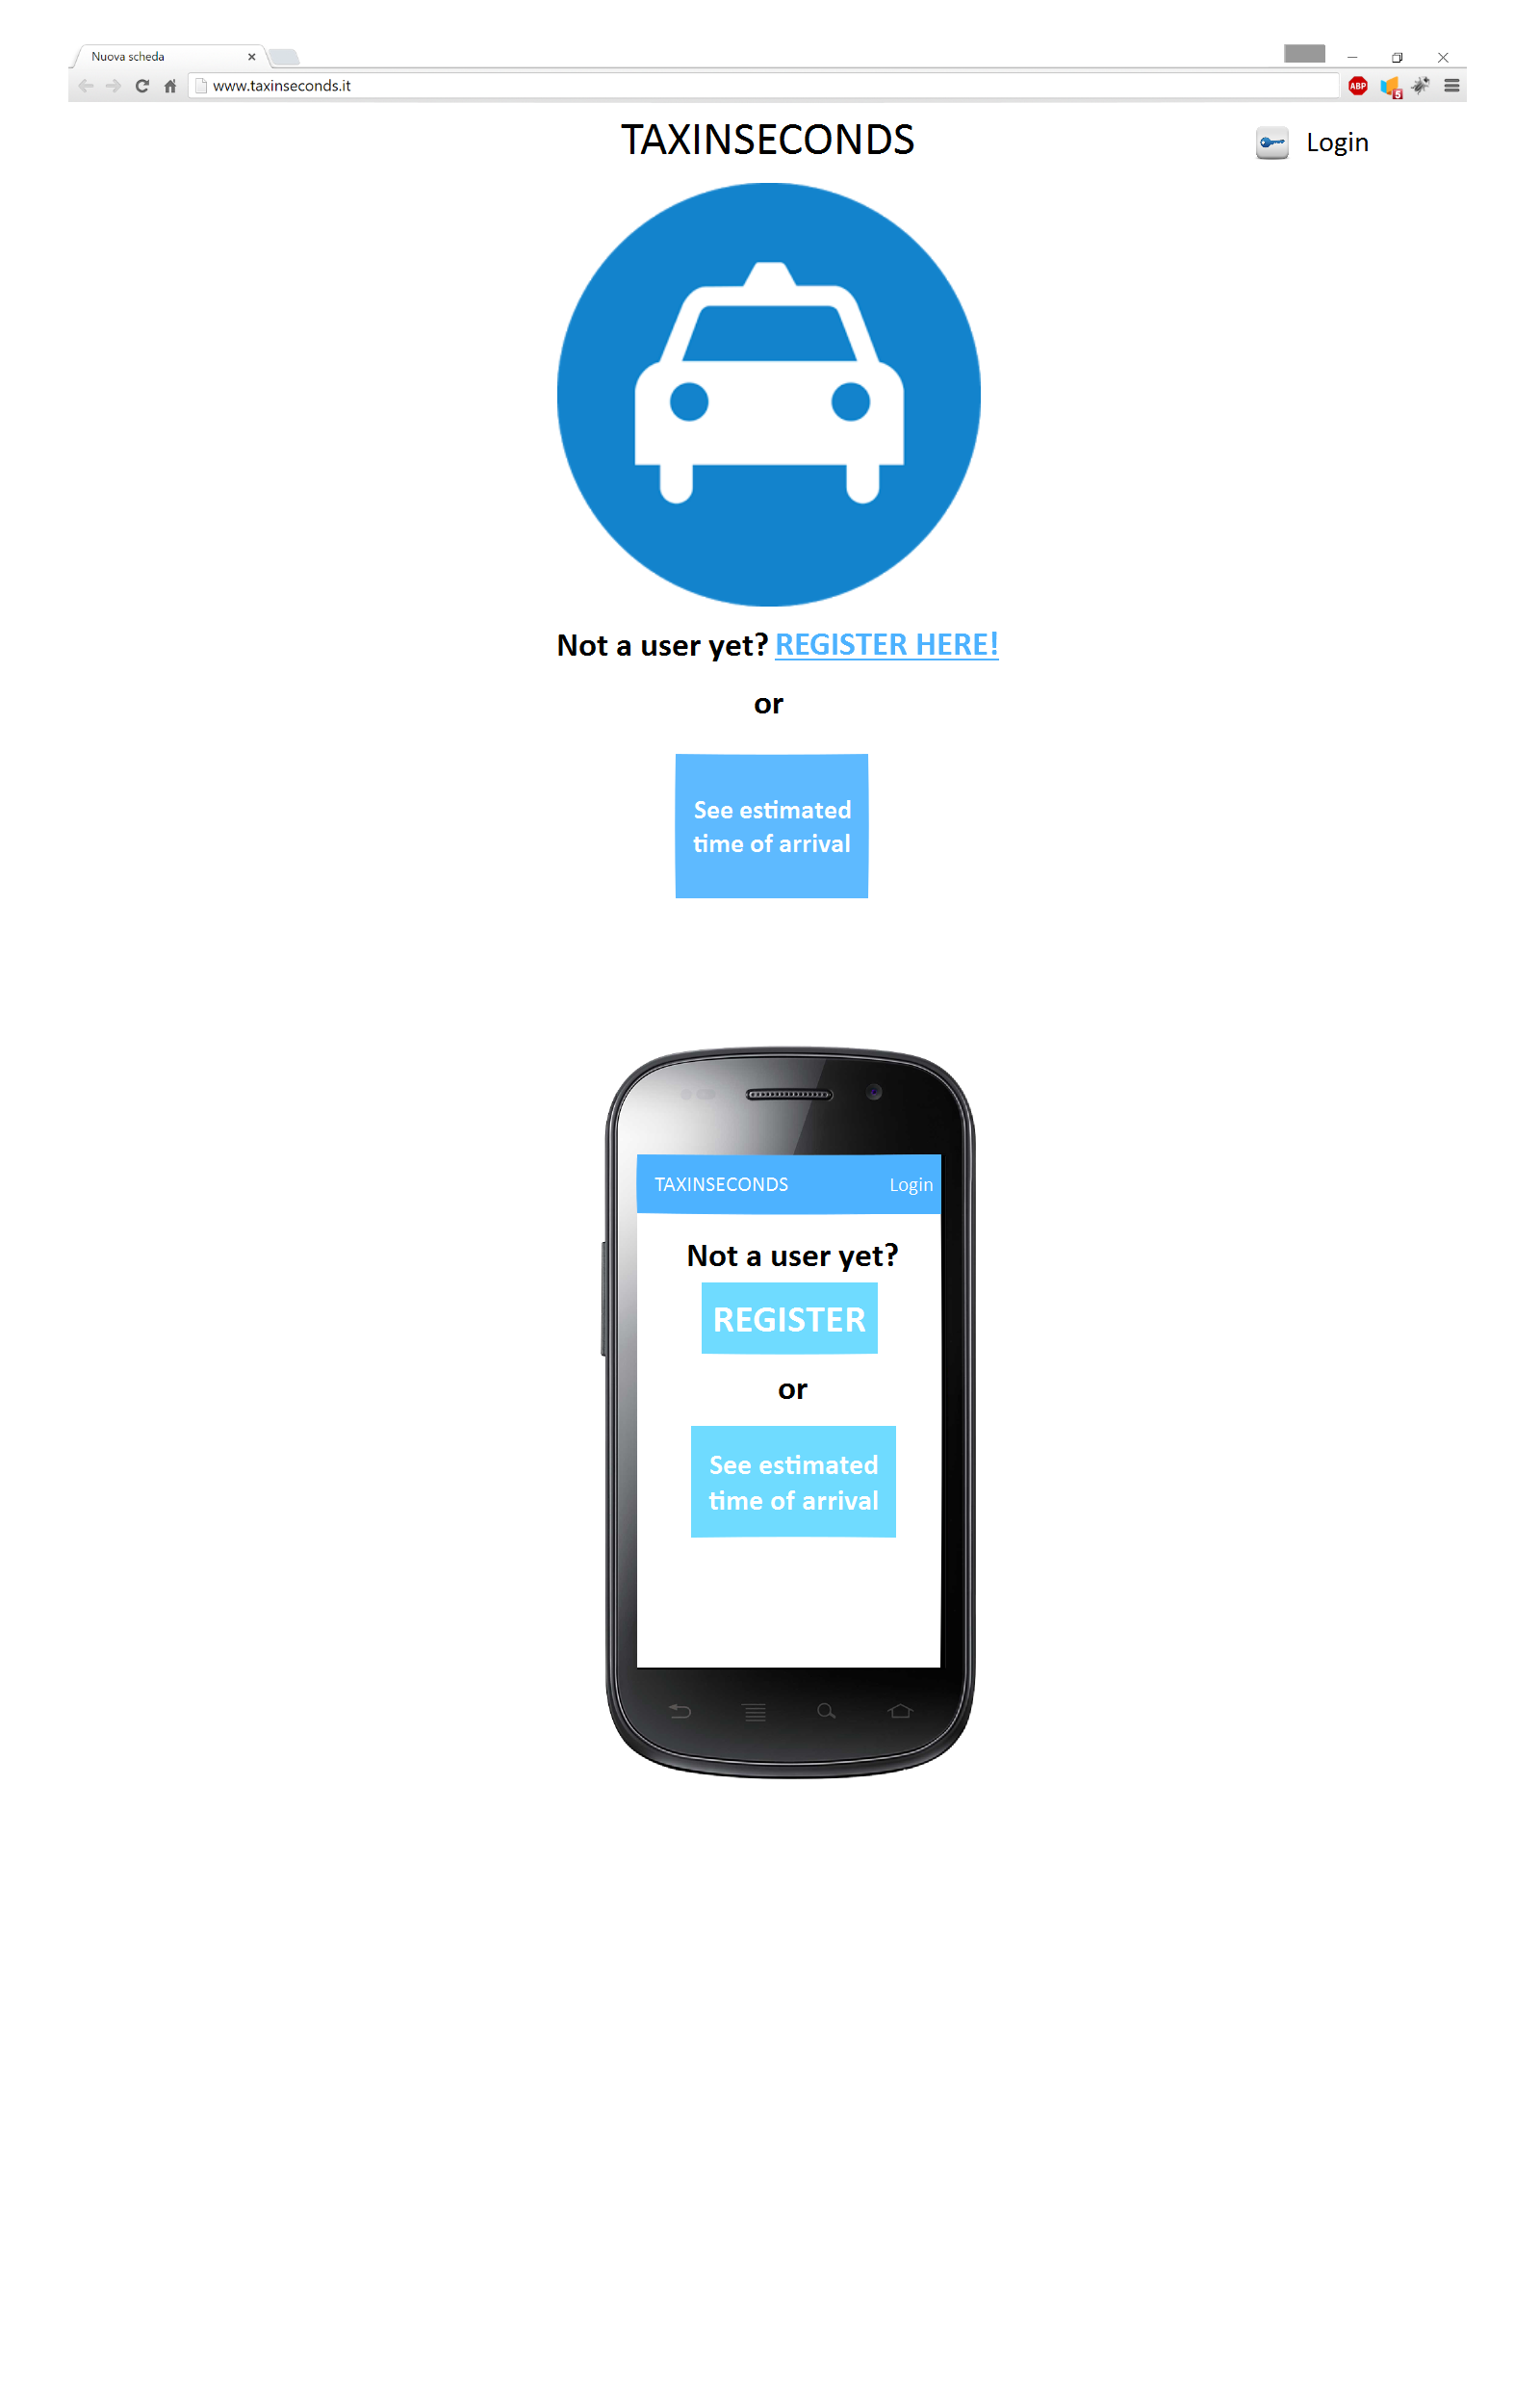
\includegraphics[width=\textwidth,height=\textheight,keepaspectratio]{GuestInterface}
	\end{center}
\end{frame}
\begin{frame}
	\frametitle{Use Cases}
	\framesubtitle{All the actions allowed were planned and analysed}
	\begin{center}
		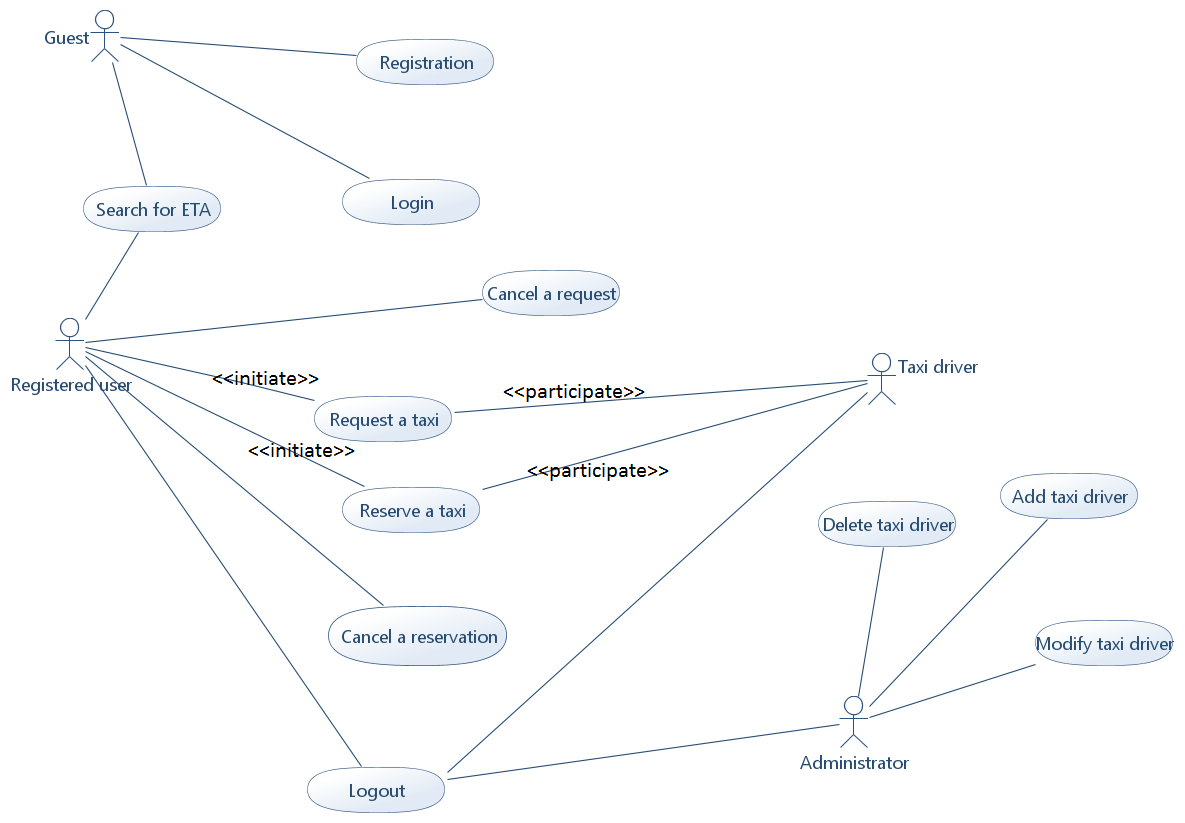
\includegraphics[width=\textwidth,height=\textheight,keepaspectratio]{UseCaseDiagram}
	\end{center}
\end{frame}
\begin{frame}
	\frametitle{Use Cases}
	\framesubtitle{Each use case is analysed in depth with a sequence diagram}
	\begin{center}
		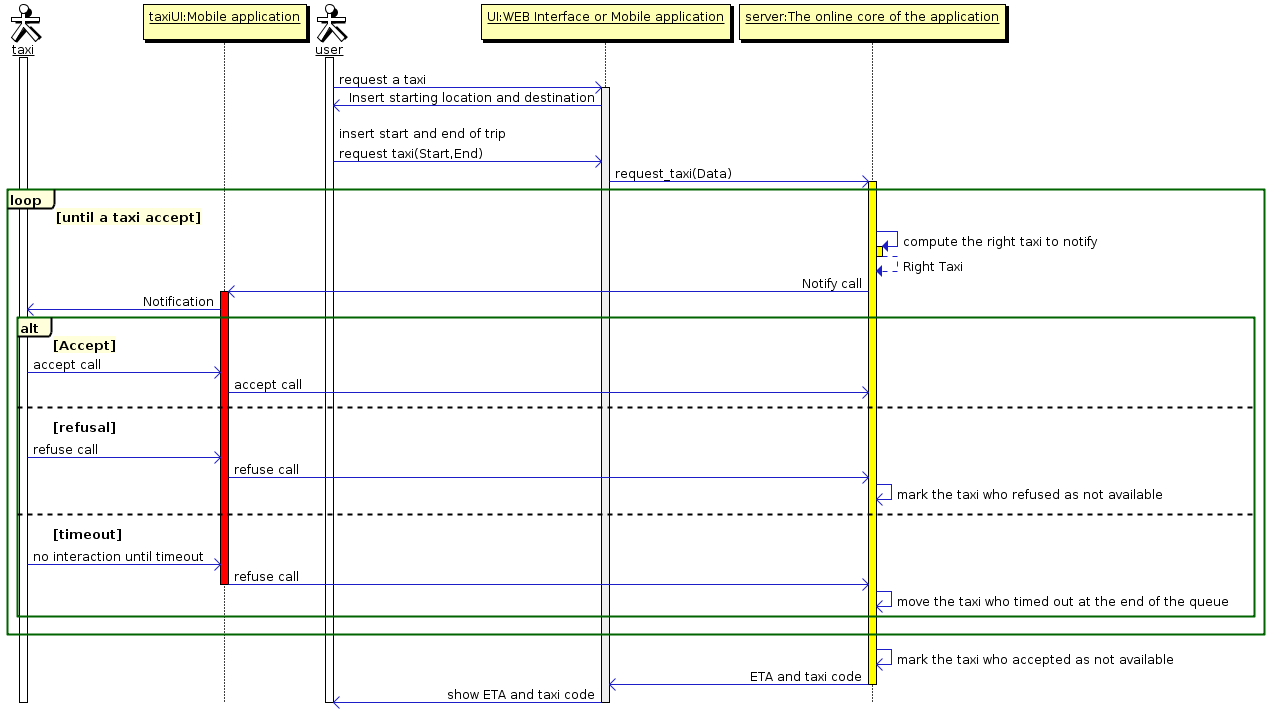
\includegraphics[width=\textwidth,height=\textheight,keepaspectratio]{request-a-taxi}
	\end{center}
\end{frame}
\begin{frame}
	\frametitle{Class Diagram}
	\framesubtitle{The class diagram was kept as readable as possible, underlying the main decisions taken}
	\begin{center}
		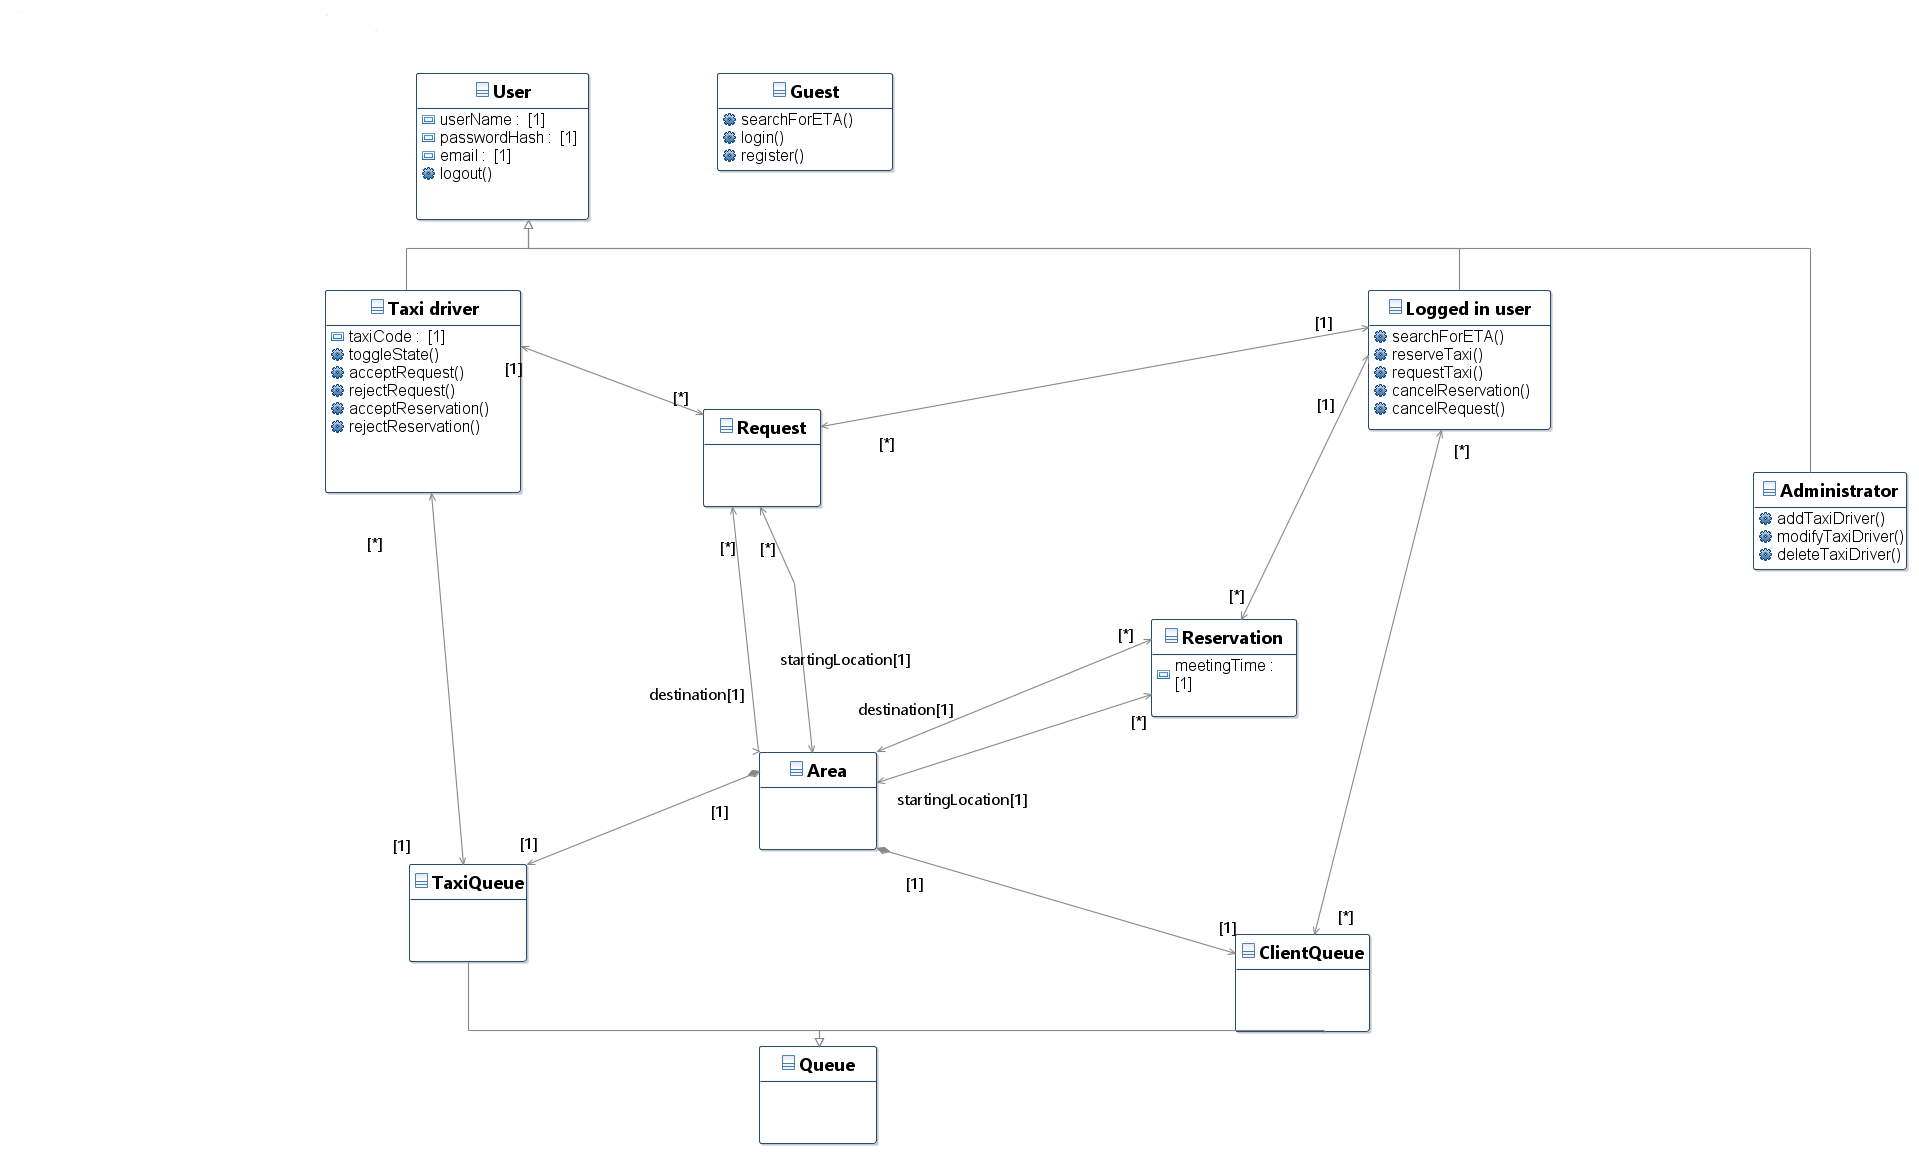
\includegraphics[width=\textwidth,height=\textheight,keepaspectratio]{ClassDiagram}
	\end{center}
\end{frame}
\begin{frame}
	\frametitle{Alloy}
	\begin{center}
		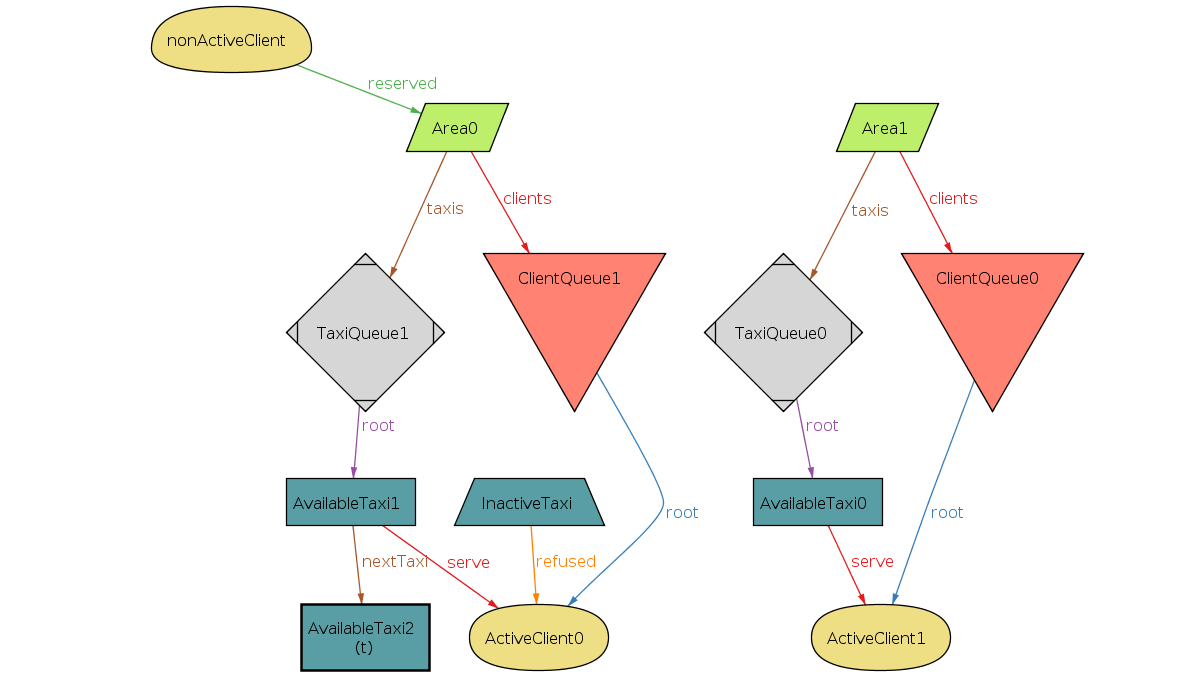
\includegraphics[width=\textwidth,height=\textheight,keepaspectratio]{reserved-and-refused}
	\end{center}
\end{frame}

\section[Section]{Design Document}
\begin{frame}
	\begin{center}
		Design Document
	\end{center}
\end{frame}
\begin{frame}
	\frametitle{The Design}
	The architecture of the application is pretty standard
	\begin{itemize}
		\item Classical DMZ structure for the Network 
		\item Database + Web server for the components
	\end{itemize}
\end{frame}
\begin{frame}
	\frametitle{The Deployment}
	\framesubtitle{A standard DMZ + Internal network approach was used}
	\begin{center}
		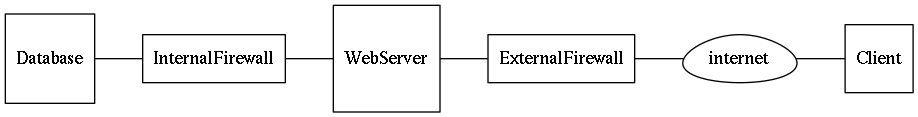
\includegraphics[width=\textwidth,height=\textheight,keepaspectratio]{dot/deployment}
	\end{center}
\end{frame}
\begin{frame}
	\frametitle{The Component View}
	\begin{center}
		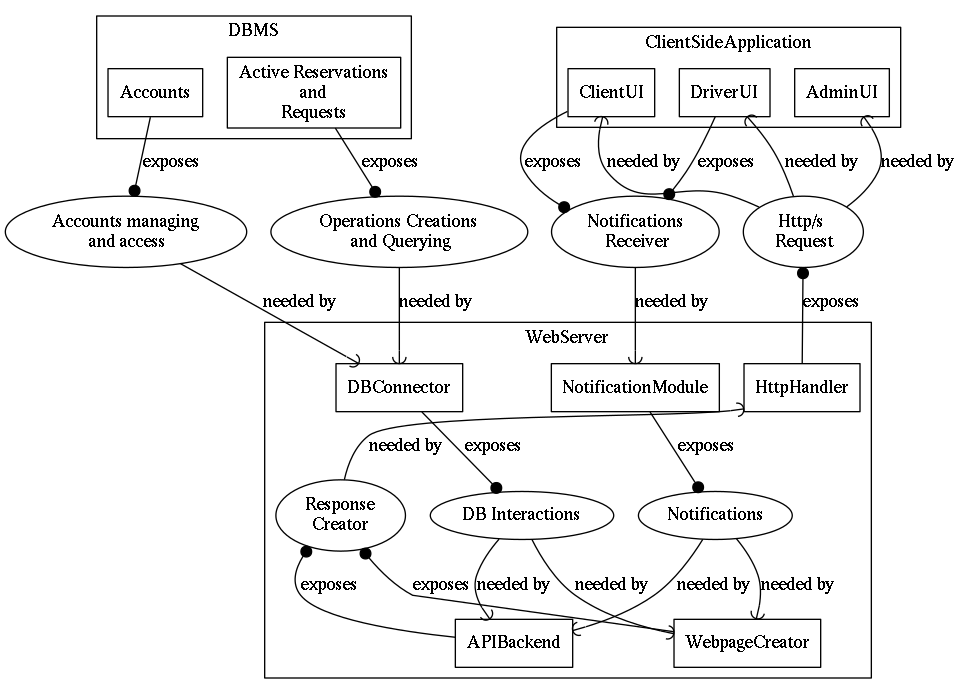
\includegraphics[width=\textwidth,height=\textheight,keepaspectratio]{dot/component}
	\end{center}
\end{frame}
\begin{frame}
	\frametitle{More on the Components}
	\framesubtitle{Extensibility and maintainability as targets}
	\begin{itemize}
		\item Both mobile and web version are based on web technologies.
		\item The queues, reservations and requests are computed by the DBMS.
		\item The web server ignores the fact that the client is using a mobile app or a browser.
		\item The APIs query the DBMS in the exact same way the Web Server does.
	\end{itemize}
\end{frame}
\begin{frame}
	\frametitle{More on the Components}
	\framesubtitle{Focus on the WebServer}
	\begin{center}
		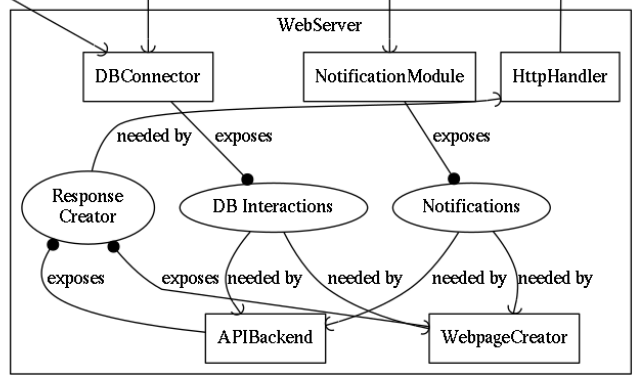
\includegraphics[width=\textwidth,height=\textheight,keepaspectratio]{dot/Webserver}
	\end{center}

\end{frame}

\section[Section]{Test Document}
\begin{frame}
	\begin{center}
		Test Document	
	\end{center}
\end{frame}
\begin{frame}
	\frametitle{The sandwich approach}
	\framesubtitle{}
	The sandwich approach allows to first test the outer parts of the applications, which are easier to test with mock data and mock requests.\\
	\-\\
	We chose to first test the UIs and the DBMS tables, in order to have a reliable surrounding when testing the WebServer part, which is the core of the application.\\
	\-\\
	Once reached the Integration of the WebServer we decided to keep the same approach even for the internal components.
\end{frame}

%\begin{frame}
%	\frametitle{The Integration Sequence}
%	\framesubtitle{}
%	%TODO erica non ho capito cosa devo fare: ``ah poi nel testing io direi di far vedere l'ordine di integrazione''
%\end{frame}

\section[Section]{Project Plan}
\begin{frame}
	\begin{center}
		Project Plan
	\end{center}
\end{frame}
\begin{frame}
	\frametitle{Function Points}
	152 FP in Total:
	\begin{itemize}
		\item Internal Logical File 45 FP
		\item External Input 70 FP
		\item External Output 19 FP
		\item External Inquiry 18 FP
	\end{itemize}
\end{frame}
\begin{frame}
	\frametitle{COCOMO}
	\framesubtitle{}
	\begin{itemize}
		\item \textasciitilde7000 estimated thousands of \textbf{S}ource \textbf{L}ines \textbf{O}f \textbf{C}ode
		\item \textasciitilde25 Person-Month
		\item 3 People for a total of 10 Months
	\end{itemize}
\end{frame}
\begin{frame}
	\frametitle{Risks}
	\framesubtitle{}
	\begin{itemize}
		\item	Personnel shortfall due to any cause (e.g. illness)
		\item	Capacity shortfalls of the entire system
		\item	Problems with the mobile application development framework
		\item	Taxi drivers don't cooperate in the use of the application
		\item	The application is not well-accepted by the public
	\end{itemize}
\end{frame}

\section[Section]{Code Inspection}
\begin{frame}
	\begin{center}
		Code Inspection
	\end{center}
\end{frame}
\begin{frame}
	\frametitle{The Checklist}
	\framesubtitle{The Style is ok}
	\begin{itemize}
		\item Naming conventions were mainly respected
		\item Braces and indention respected the standard except for a couple of lines
		\item File organization and white spaces were correctly used. With the exception of a comment line that was too long and a couple of white lines to be removed.
		\item High level breaks were used in code lines
	\end{itemize}
\end{frame}
\begin{frame}
	\frametitle{The Checklist}
	\framesubtitle{But the style is not everything}
	Documentation is mostly absent or incomplete\\
	\-\\
	There is a condition of an if that was commented out with no reasons to explain why\\
	%TODO  gli esempi del codice commentato via non riesco a metterlo
	\-\\
	One of the functions was definitely too complex, it represented the logical function of three different methods, one after the other, separated by a comment.\\
	An other couple should have been splitted in at least two simpler ones.
\end{frame}
\begin{frame}
	\frametitle{The Checklist}
	\framesubtitle{A couple of exceptions}
	A couple of exceptions were caught but not handled, and both of them have a comment stating\\
	\-\\
	\texttt{{\color{Blue}try }\{\\\-	reader.close();\\\} {\color{Blue}catch} (Exception e) \{\\{\color{Green}\-	//ignore?}\\\}}
\end{frame}

\begin{frame}
	\frametitle{To close up}
	\framesubtitle{Closing is important}
	There is a method that opens a list of inputstreams from an archive file and if an exception is thrown the handler \underline{just closes the last inputstream} opened.\\
	\-\\
	According to the Java Documentation closing \underline{every} inputstream that refers to a file closes the file itself.\\
	\-\\
	Even if a failure in that point of the application probably implies a failure of the whole process, that will soon close and free the file descriptors, this is a terrible practice and it should be avoided.
\end{frame}
\begin{frame}
	\frametitle{}
	\framesubtitle{}
	{\Huge
		\begin{center}
			That's all!
		\end{center}
	}
\end{frame}
\end{document}

